\nocite{*}

\chapter{Библиография} \label{bibliography}

Список литературы, приведенный ниже, составлен без претензий на полноту представления тем, указанных в заголовках, и без претензий на полноту подкрепления материала, изложенного в основной части курса. В библиографии указаны некоторые из "центральных" работ и описаний методов, традиционно упоминаемых при обсуждении материалов в перечисленных темах. Но также, при составлении библиографии, в рамках некоторых тем, упомянуты материалы, относящиеся к теме, но при этом несколько расширяющие принятые там постановки вопросов. "Новое - это хорошо забытое старое", и часто для этого оказывалось достаточно вспомнить некоторые давно "вышедшие из моды" направления исследований. 
%И еще, намерением при этом было вспомнить некоторых людей, котоых можно отнести к "учителям", и некоторые их идеи. Не со всеми из них мы были знакомы лично, но про многих из них удалось узнать не по официальным хроникам, а из разговоров и при общении с коллегами.


\selectlanguage{english}

\section{Структурная биоинформатика}


\addtocategory{bib_m_structural}{Фейнман_eng,Morse_eng,Wirth_eng,Kernighan_1978,Stroustrup_1985,Hollup_2005,Skjærven_2014,Olsson_2011,Pettersen_2004,Brooks_2009,Berendsen_1984,Onufriev_2002,MacKerell_1998,Cornell_1995,Xiang_2006,Yang_2015,Wang_2008,Xu_2006,Sali_1993,Moult_2016,g09,Valiev_2010,Schmidt_1993,Kelley_2009,Brozell_2012,Jain_2009,Goodsell_1990,Trott_2010,Das_2008,Tovchigrechko_2006,Bultinck_2002,Duan_2003,Alder_1957,Verlet_1967,Case_2005,Finkelstein_1994,Karplus_1997,Galaktionov_2001,McCammmon_1977,Liwo_2005,Connaughton_2004,Ngo_1992,Orengo_1993,Efimiv_1994,Tsai_2000,Bellman_1952,Balevicius_2010,DeMarco_2014,Feranchuk_2016,Feranchuk_1995,Skoromnik_2017}

\addtocategory{bib_m_structural_rus}{Ландау_1,Ландау_2,Ландау_3,Ландау_5,Фейнман_rus,Морс_1,Морс_2,Вирт_1982,Керниган_1992,Холмодуров_2003,Хохлов_2009,Гуреев_2018,Козырев_2010,Финкельштейн_2012,Андрианов_2013}


\bibparheader{Теоретическая физика - учебники} 

\selectlanguage{russian} \cite{Ландау_1,Ландау_2,Ландау_3,Ландау_5,Фейнман_rus,Морс_1,Морс_2};\selectlanguage{english}  \cite{Фейнман_eng,Morse_eng}

\bibparheader{Программирование - "классические" учебники}

\selectlanguage{russian} \cite{Вирт_1982,Керниган_1992};\selectlanguage{english} \cite{Wirth_eng,Kernighan_1978,Stroustrup_1985}.

\bibparheader{Квантовые расчеты} 

Силовые поля и парциальные заряды: \cite{Gasteiger_1980,Mulliken_1955,Jakalian_2000,Hehre_1969}.

Пакеты программ: Gaussian \parencite{g09}, GAMESS \parencite{Schmidt_1993}, NWChem \parencite{Valiev_2010}.

\bibparheader{Анализ нормальных мод}: \cite{Skjærven_2014,Hollup_2005}

\bibparheader{Молекулярная динамика}

\selectlanguage{russian} 
Учебники и пособия на русском: \cite{Холмодуров_2003,Хохлов_2009}.

\selectlanguage{english} 
Теория, классические работы, обоснование методов и подходов: \cite{Alder_1957,Verlet_1967,Berendsen_1984,Cornell_1995,Bultinck_2002,Bonvin_2010,Андрианов_2013}.

Пакеты программ: Amber \parencite{Case_2005}, Charmm \parencite{Brooks_2009}.

\bibparheader{Уравнение Пуассона-Больцмана и учет растворителя}: \cite{Berendsen_1981,Onufriev_2002,Olsson_2011,Hou_2011,}

\bibparheader{Моделирование структуры белков}:

Учебный курс: \cite{Финкельштейн_2012}

Теория, классические работы, обоснование методов и подходов: \cite{Finkelstein_1994,Karplus_1997,Galaktionov_2001,McCammmon_1977,Liwo_2005}

Расчеты боковых цепей: \cite{Wang_2008,Xu_2006}

Моделирование "по гомологии": Modeller \parencite{Sali_1993}, Jackal/Nest \parencite{Xiang_2006}, Phyre \parencite{Kelley_2009}

Моделирование "de novo": Tasser \parencite{Yang_2015}, Rosetta \parencite{Das_2008}

"Эксперимент" CASP и сравнение методов: \cite{Moult_2016}

Пути сворачивания белка: \cite{Connaughton_2004,Ngo_1992,Orengo_1993,Efimiv_1994,Tsai_2000,Козырев_2010,Bellman_1952}

\bibparheader{Молекулярный докинг}: 

Докинг лигандов: Autodock \parencite{Goodsell_1990}, Autodock Vina \parencite{Trott_2010}, UCSF Dock \parencite{Brozell_2012}, Surflex \parencite{Jain_2009}.

Докинг белков: \cite{Tovchigrechko_2006}

Пособие с описанием методов: \cite{Гуреев_2018}

\bibparheader{Визуализация и компьютерная графика}: UCSF Chimera \parencite{Pettersen_2004}, VMD \parencite{Humphrey_1996}.

\bibparheader{Некоторые прикладные работы по структурной биоинформатике и смежным темам}: \cite{Balevicius_2010,DeMarco_2014,Feranchuk_2016,Feranchuk_1995,Skoromnik_2017} 

\selectlanguage{russian}

\biblistheader{публикации и издания к главе, на русском}

\printbibliography[heading=none,category=bib_m_structural_rus]

\selectlanguage{english}

\biblistheader{публикации и издания к главе, на английском}

\printbibliography[heading=none,category=bib_m_structural]


\section{Системная биоинформатика}

\addtocategory{bib_m_system}{Lefort_2015,Katoh_2013,Tatusov_1994,Altschul_1990,Edgar_2004,Larkin_2007,Bankevich_2012,Luo_2012,Simpson_2009,Kurtz_2004,Trapnell_2012,Li_2011,Robinson_2010,Anders_2010,Cox_2011,Röst_2016,Craig_2004,Vaudel_2011,Lander_1988,Langmead_2009,Grabherr_2011,McDonald_2012,Cole_2014,Edgar_2010,Drummond_2012,Sanderson_2002,Drummond_2012,Stamatakis_2006,Guindon_2003,Huelsenbeck_2001,Tamura_2007,Schloss_2009,Caporaso_2010,Kopylova_2016,Oksanen_2007,Leontovich_2002,Schiffels_2014,Needleman_1970,Smith_1981,Burrows_1994,Idury_1995,Fitch_1967,Felsenstein_1981,Chen_2016,Anglicheau_2009,Sanderson_2002,Drummond_2006,Svirezhev_2000,Feigenbaum_1983,DeGrandi_2010,Yakovenko_2009,Xu_2017,Harte_2001,Higuchi_1988,Jelinek_1998,Karbauskaite_2016,Mandelbrot_1960,Mandelbrot_1967,Peng_1994,Richardson_1961,Seuront_2015,Sornette_2002,Rak_2007,Whittaker_1960,Hill_1973,Jost_2006,Chiu_2014,Chao_2014,Wittebole_2009,Eliazar_2012,Marrugan_2004,Preston_1948,McGill_2007,Belikov_2005,Marchenkov_2018,Hebb_1949,Rosenblatt_1957,Kohonen_1982,Hopfield_1985,Lodish_2000,Picciotto_2012,Belousov_2001,Irving_1992,Sum_1999,Yao_2019,Nazıroğlu_2014,Cui_2013,Didelot_2015,Duchêne_2016}

\begin{figure}[H]
  \centering
  \vskip 12pt 

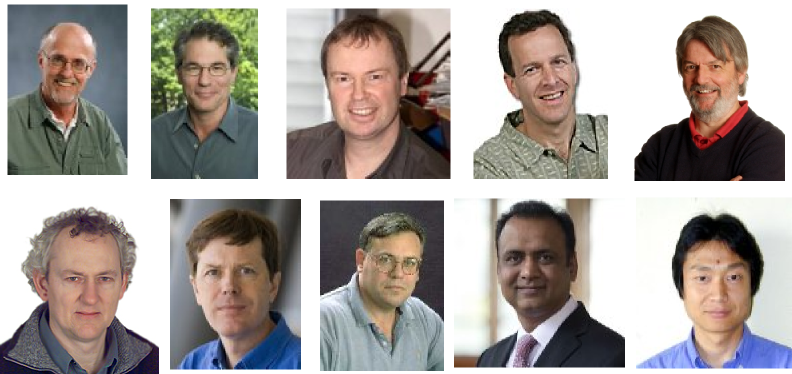
\includegraphics [width=0.85\linewidth]{bioinformaticians.png}
  \vskip 12pt
  \caption[m1]{
\textbf{Некоторые из современных биоинформатиков}\itshape

10 наиболее цитируемых современных специалистов по биоинформатике (по версии системы Google Scholar, декабрь 2018 г.)
\\
 \fontsize{11pt}{11pt}\selectfont
  Верхний ряд: W.Miller, G.Myers, P.Bork, S.Salzberg, D.G.Higgins; Нижний ряд: T.J.Gibson, R.Durbin, S.Altschul, S.Kumar, K.Tamura.
  Из них, W.Miller, G.Myers, S.Altschul - соавторы статьи с представлением программы Blast (1990), P.Bork, S.Salzberg, R.Durbin - участники проектов по определению генома человека (2001), D.G.Higgins, T.J.Gibbson - соавторы статьи с описание пакета Clustal-W (1994), S.Kumar, K.Tamura - соавторы статьей с описанием пакета MEGA (версии 1-7, 1994-2007).
}
 \label{img:bioinformaticians}
\end{figure}

\addtocategory{bib_m_system_rus}{Владыко_2012,Владыко_2001,ТимофеевРесовский_1969,Ризниченко_2003,Марчук_1991,Остапеня_1985}

\bibparheader{Выравнивание последовательностей}

Алгоритмы и "классические" работы: \cite{Needleman_1970,Smith_1981,Burrows_1994,Tatusov_1994,Leontovich_2002}.

Пакеты программ: Blast \parencite{Altschul_1990}, Mafft \parencite{Katoh_2013}, Muscle \parencite{Edgar_2004}, Clustal \parencite{Larkin_2007}, Mummer \parencite{Kurtz_2004}, Bowtie \parencite{Langmead_2009}, UBlast \parencite{Edgar_2010}. 

\bibparheader{Ассемблирование}

Алгоритмы и "классические" работы: \cite{Lander_1988,Idury_1995}.

Пакеты программ:  Abyss \parencite{Simpson_2009}, SOAPdenovo \parencite{Luo_2012}, Spades \parencite{Bankevich_2012}.

\bibparheader{Обработка экспериментов по масс-спектрометрии}

Пакеты программ: Tandem \parencite{Craig_2004}, Andromeda \parencite{Cox_2011}, OpenMS \parencite{Röst_2016}, SearchGUI \parencite{Vaudel_2011}.

Некоторые прикладные работы: \cite{Pradke_2017,Holland_2014}

\bibparheader{Обработка экспериментов RNA-Seq}

Алгоритмы и программы с их реализацией: RSEM \parencite{Li_2011}, DeSeq \parencite{Anders_2010}, edgeR \parencite{Robinson_2010}

Пакеты программ с "технологическими процессами":  Tophat/Cufflinks \parencite{Trapnell_2012}, TrinityRNASeq \parencite{Grabherr_2011}.

Сравнение методов и прикладные работы: \cite{Anglicheau_2009,Chen_2016,Won_2014,Adamska_2007,Anavy_2014,Levin_2016}

\bibparheader{Обработка данных в медицине}

Обзорные работы: \cite{Rattan_2006,Wu_2016,deSouza_2015,Cumming_2009}

\bibparheader{Модели в вычислительной биологии}

Издания и учебники на русском: \cite{ТимофеевРесовский_1969,Марчук_1991,Ризниченко_2003}

Некоторые из работ с обобщениями моделей: свойства детерминированного хаоса \parencite{Feigenbaum_1983}, связи биологических моделей и статистической физики \parencite{Svirezhev_2000}, универсальная модель квантового перехода \parencite{DeGrandi_2010}

Математическая экология, классические работы, сравнение и обобщение методов: \cite{Preston_1948,Whittaker_1960,Hill_1973,Marrugan_2004,Jost_2006,McGill_2007,Wittebole_2009,Eliazar_2012,Chiu_2014,Chao_2014}

Некоторые из прикладных работ по смежным темам: \selectlanguage{russian}\cite{Остапеня_1985,Владыко_2001,Владыко_2012}; \selectlanguage{english}\cite{Belikov_2005,Marchenkov_2018}

\bibparheader{Нейронные сети}

Классические работы: \cite{Hebb_1949,Rosenblatt_1957,Kohonen_1982,Hopfield_1985}

К модели сети с двумя уровнями возбуждения: \cite{Lodish_2000,Picciotto_2012,Belousov_2001,Irving_1992,Paulus_2016,BenAri_2014,Sum_1999}

\bibparheader{Теория фракталов}

Классические работы: \cite{Mandelbrot_1960,Mandelbrot_1967,Peng_1994,Richardson_1961,Higuchi_1988}

Обзорные работы и сравнение методов: \cite{Harte_2001,Jelinek_1998,Karbauskaite_2016,Seuront_2015}

Некоторые из расширений и обобщений подходов: \cite{Yakovenko_2009,Xu_2017,Sornette_2002,Rak_2007}

\bibparheader{Эволюция и филогенетические деревья}

Теория, классические работы, обоснование методов и подходов: \cite{Fitch_1967,Sanderson_2002,Felsenstein_1981,Drummond_2006}.

Пакеты программ: Beast \parencite{Drummond_2012}, RaxML \parencite{Stamatakis_2006}, FastME \parencite{Lefort_2015}, PhyML \parencite{Guindon_2003}, MrBayes \parencite{Huelsenbeck_2001}, MEGA \parencite{Tamura_2007}.

Некоторые из прикладных работ: \cite{Cui_2013,Didelot_2015,Duchêne_2016,Mironova_2018,Потапова_2018}

\bibparheader{Метагеномика}

Обоснование и сравнение методов, подходов и алгоритмов: \cite{McDonald_2012}

Пакеты программ: QIIME \parencite{Caporaso_2010}, Mothur \parencite{Schloss_2009}, SortmeRNA \parencite{Kopylova_2016}, RDP \parencite{Cole_2014}, Vegan \parencite{Oksanen_2007}.

\selectlanguage{russian}

\biblistheader{публикации и издания к главе, на русском}

\printbibliography[heading=none,category=bib_m_system_rus]

\selectlanguage{english}

\biblistheader{публикации и издания к главе, на английском}

\printbibliography[heading=none,category=bib_m_system]

\addtocategory{bib_authors_rus}{Феранчук_2006,Потапов_2011,Потапова_2018}

\addtocategory{bib_authors}{Brodsky_1992,Feranchuk_2010,Feranchuk_2007,Mukha_2011,Potapova_2012,Mironova_2018,Potapova_2018,Feranchuk_2018a,Feranchuk_2018b,Kuzmin_2019}

\selectlanguage{russian}

\biblistheader{публикации и издания авторов, на русском и белорусском}

\printbibliography[heading=none,category=bib_authors_rus]

\selectlanguage{english}

\biblistheader{публикации и издания авторов, на английском}

\printbibliography[heading=none,category=bib_authors]
